%%%%%%%%%%%%%%%%%%%%%%%%%%%%%%%%%%%%%%%%%%%%%%%%%%%%%%%%%%%%%%%%%%%%%%%%%%%%%%%%
% TUM-Vorlage: Präsentation - Beispiele
%%%%%%%%%%%%%%%%%%%%%%%%%%%%%%%%%%%%%%%%%%%%%%%%%%%%%%%%%%%%%%%%%%%%%%%%%%%%%%%%


%%%%%%%%%%%%%%%%%%%%%%%%%%%%%%%%%%%%%%%%%%%%%%%%%%%%%
%% Folie: Gültigkeit der Masterfolien              %%
%%%%%%%%%%%%%%%%%%%%%%%%%%%%%%%%%%%%%%%%%%%%%%%%%%%%%

%%%%%%%%%%%%%%%%%%%%%%%%%%%%%%%%%%%%%%%%%%%%%%%%%%%%%
%% Folie: Grundlage der Masterfolien               %%
%%%%%%%%%%%%%%%%%%%%%%%%%%%%%%%%%%%%%%%%%%%%%%%%%%%%%

%%%%%%%%%%%%%%%%%%%%%%%%%%%%%%%%%%%%%%%%%%%%%%%%%%%%%
%% Folie: 2-zeilige Überschrift                    %%
%%%%%%%%%%%%%%%%%%%%%%%%%%%%%%%%%%%%%%%%%%%%%%%%%%%%%


%%%%%%%%%%%%%%%%%%%%
%%%%%%%%%%%%%%%%%%%%
\begin{frame}
    \shiftedframetitle{Content}
    
    \begin{enumerate}
    \item Shallow Water Equations model \vspace{0.5cm}
    \item Scope of this thesis\vspace{0.5cm}
    \item Tools\vspace{0.5cm}
    \item Current status\vspace{0.5cm}
    \item TO-DOs
    \end{enumerate}



\end{frame}
\clearpage


%%%%%%%%%%%%%%%%%%%%
%%%%%%%%%%%%%%%%%%%%
\begin{frame}
    \shiftedframetitle{Shallow Water Equations (SWE) model}
\vspace{-3mm}
\begin{itemize}
\item<2-> Starting with Navier-Stokes Equation for \textbf{incompressible inviscid} flow(\ref{ns}) and \textbf{mass continuity law}(\ref{cont})
\begin{align}
\frac{\partial u}{\partial t} + u\frac{\partial u}{\partial x} + v\frac{\partial u}{\partial y} + w\frac{\partial u}{\partial z} &= - \frac{\partial p}{\partial x} \nonumber \\ 
\frac{\partial v}{\partial t} + u\frac{\partial v}{\partial x} + v\frac{\partial v}{\partial y} + w\frac{\partial v}{\partial z}&= - \frac{\partial p}{\partial y} \label{ns} \\ 
\frac{\partial w}{\partial t} + u\frac{\partial w}{\partial x} + v\frac{\partial w}{\partial y} + w\frac{\partial w}{\partial z} &= - \frac{\partial p}{\partial z} + g \nonumber\\[0.3cm]
\frac{\partial u}{\partial x} + \frac{\partial v}{\partial y} + \frac{\partial w}{\partial z} &= 0 \label{cont}
\end{align}

\item<3-> First assumption:
  $L \ll H$, which from (\ref{cont}) it leads to $u,v\ll w$. Second assumption: \myBlu{vertical momentum exchange is negligible}. This leads to
\begin{align}
\frac{\partial u}{\partial t} + u\frac{\partial u}{\partial x} + u\frac{\partial v}{\partial y} + u\frac{\partial w}{\partial z} &= - \frac{\partial p}{\partial x} \nonumber \nonumber \\ 
\frac{\partial v}{\partial t} + v\frac{\partial u}{\partial x} + v\frac{\partial v}{\partial y} + v\frac{\partial w}{\partial z}&= - \frac{\partial p}{\partial y} \nonumber \\ 
\myBlu{0} &\myBlu{ = - \frac{\partial p}{\partial z} + g} \label{press}
\end{align}
which provides a \myBlu{solution for the pressure} as a function of the sea floor elevation and water level, see figure \ref{fig:swechem}.
\end{itemize}
\end{frame}
\clearpage


%%%%%%%%%%%%%%%%%%%%
%%%%%%%%%%%%%%%%%%%%
\begin{frame}
    \shiftedframetitle{Shallow Water Equations (SWE) model {\small(cont.)}}
\vspace{-3mm}
\begin{itemize}
\item<1-> From (\ref{cont}), we can carry out a \myOra{depth-averaged integration} on the \myOra{continuity equation}, that is 
\begin{align}
\myOra{\int_a^b} (\frac{\partial u}{\partial x} + \frac{\partial v}{\partial y} + \myOra{\frac{\partial w}{\partial z}})\ \myOra{dz} &= 0 \nonumber \\[0.2cm]
\myOra{\frac{\partial h}{\partial t}} + \frac{\partial hu}{\partial x} + \frac{\partial hv}{\partial y} &= 0
\end{align}
\item<2-> Lastly, from (\ref{ns}) and making use of \myRed{\textit{Leibnitz Integral Rule}, depth-averaged integration} on the \myRed{momentum equation}, some kinematic boundary conditions on the water surface \cite{depthAv}, and from (\ref{press}), we get the model for SWE
\begin{align}
\frac{\partial \myRed{hu}}{\partial t} + \frac{\partial}{\partial x}(\myRed{hu^2} + \myBlu{\frac{1}{2}\rho g h^2}) + \frac{\partial \myRed{huv}}{\partial y} &= \myBlu{- gh\frac{\partial b}{\partial x}} \\
\frac{\partial \myRed{hv}}{\partial t} + \frac{\partial \myRed{huv}}{\partial x} + \frac{\partial}{\partial y}(\myRed{hv^2} + \myBlu{\frac{1}{2}\rho g h^2})&= \myBlu{- gh\frac{\partial b}{\partial y} }
\end{align}
\end{itemize}
\end{frame}
\clearpage

%%%%%%%%%%%%%%%%%%%%
%%%%%%%%%%%%%%%%%%%%
\begin{frame}
    \shiftedframetitle{Shallow Water Equations (SWE) model {\small(final)}}
\vspace{-2mm}
\begin{multicols}{2}
\begin{itemize}
\item[] SWE model can be represented in a matrix form \dots
% derived from mass and momentum conservation laws, and depth averaging \dots %also derived by vertical averaging from the 3d incompressible ns eqs
\begin{align*}
\vspace{-15pt}
\begin{bmatrix}[1.3]
h\\
hu\\
hv\\
\end{bmatrix}_t \ + \ 
\begin{bmatrix}[1.0]
hu\\
hu^2 + \frac{1}{2}gh^2\\
huv\\
\end{bmatrix}_x\ &+ \ 
\begin{bmatrix}[1.0]
hv\\
huv\\
hv^2 + \frac{1}{2}gh^2\\
\end{bmatrix}_y = 
\begin{bmatrix}[1.0]
0\\
-ghb_x\\
-ghb_y
\end{bmatrix}\\[2em]
\frac{\partial q}{\partial t} + \dfrac{\partial F(q)}{\partial x} + &\frac{\partial G(q)}{\partial y} = S(q,x,y,t) 
\end{align*}
\vspace{5pt}
\item[]
\begin{figure}
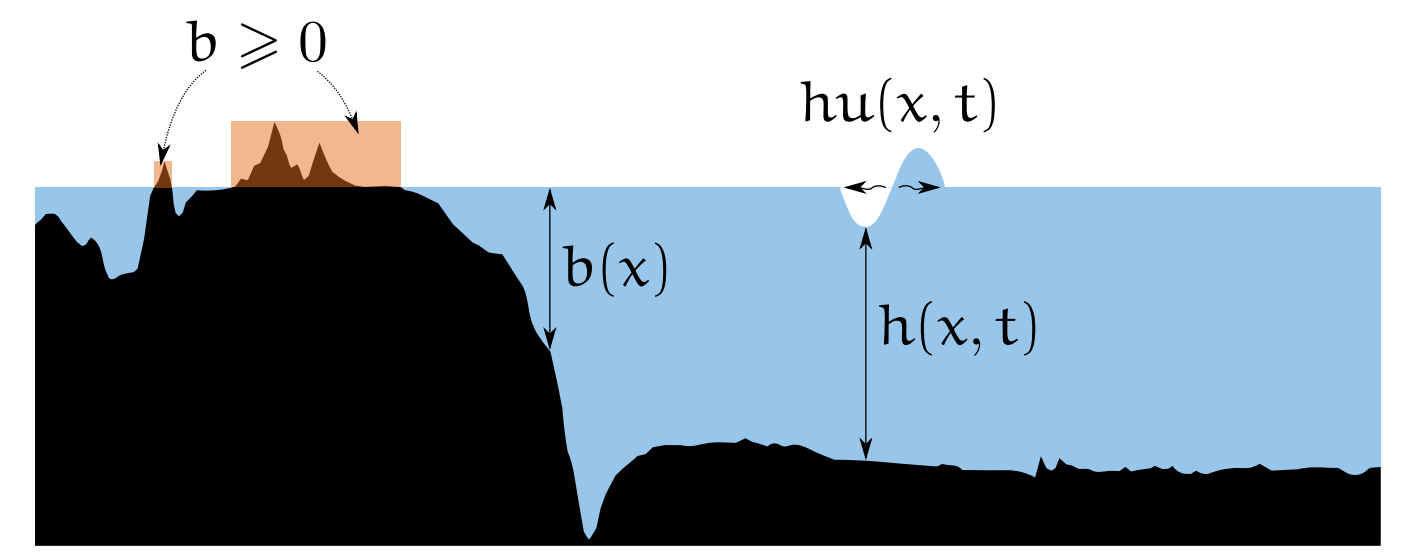
\includegraphics[scale=0.2]{./Resources/Images/swe.png}%
\caption{SWE variables schematic \footnote{\url{https://www5.in.tum.de/SWE/lugano2013/swe_anatomy.pdf}}}
\label{fig:swechem}
\end{figure}
\end{itemize}

\vfill\columnbreak

\begin{itemize}
\setlength\itemsep{2em}
\item<2->[] The \textbf{\myGre{Shallow Water Equations}} \dots
\item<3-> \myGre{neglect vertical velocity};  $ W \ll U,V $, since horizontal distances $L$ $\gg$ vertical distance $H$
\item<4-> simplify \myGre{$3D$} Navier-Stokes \myGre{to} a \myGre{$2D$} system of equations
\item<5-> represent a \myGre{hyperbolic PDE} system $\rightarrow$ \myGre{Riemann} Problem and \myGre{FVM}
\item<6-> Applications: {\small \myGre{Free surface} flows around structures, tsunamis prediction, atmospheric flows, \dots}
\end{itemize}
\end{multicols}

\end{frame}
\clearpage

%%%%%%%%%%%%%%%%%%%%%%%%%%
%%%%%%%%%%%%%%%%%%%%%%%%%%

\begin{frame}
\shiftedframetitle{Scope of this thesis}

\begin{multicols}{2}
\begin{itemize}
\item<2->[]    
 \hspace{0.35\columnwidth}{\large\textbf{Background}}
 \vspace{3em}
 \begin{itemize}
  \setlength\itemsep{2em}
  \item  full description of \myBlu{\textit{shallowFOAM}}  solver for \myBlu{$2D$} SWE \cite{mintgen}
 \item  \myBlu{coupling $2D$} SWE and \myBlu{$3D$} RANS solvers $\rightarrow$ development of \textit{shallowInterFOAM} \cite{mintgen}
 \item BSc. Christiaan Osse implemented \cite{mintgen} with \myBlu{\textit{preCICE}}
 \end{itemize}
    
\vfill\columnbreak

\item<3->[]
\hspace{0.35\columnwidth}{\large\textbf{Goals}}
\vspace{3em}
 \begin{itemize}
    \setlength\itemsep{2em}

 \item<4-> \myCRed{Extend} \cite{mintgen} coupling ($2D$ $\Longleftrightarrow$ $3D$) as a \myCRed{flexible} approach to SWE solvers
 \item<5-> Test Case: $2D$ SWE solver \& OpenFOAM 
 \item<6-> \myCRed{Coupling} \& \myCRed{Mapping} data from/to all setups: \vspace{0.4cm}
\begin{table}[]
\begin{tabular}{|lll|}\hline
$2D$ SWE       & $\rightarrow$ & $2D$ SWE       \\ \hline
$2D$ SWE       & $\rightarrow$ & $3D$ OpenFOAM \\ \hline
$3D$ OpenFOAM & $\rightarrow$ & $2D$ SWE       \\ \hline
$3D$ OpenFOAM & $\rightarrow$ & $3D$ OpenFOAM \\ \hline
\end{tabular}
\caption{Mapping setups}
\label{table:1}
\end{table}
\item<7-> \textbf{\textit{\myCRed{Extend preCICE} adapter for handling $3D$ domains}}
\end{itemize}
\end{itemize}
\end{multicols}


\end{frame}


%%%%%%%%%%%%%%%%%%
%%%%%%%%%%%%%%%%%%

\begin{frame}
	\shiftedframetitle{Tools}
 	
\begin{multicols}{2}
\begin{itemize}
 \setlength\itemsep{10pt}

\item<2->[]
\textbf{Shallow Water Equations Solver - {\small Wave-propagation method.}}
\begin{itemize}
\vspace{5pt}
 \setlength\itemsep{6pt}
\item Modified Wave-Propagation Method $\rightarrow$ \myRed{\textit{F-Wave}} \cite{levequeArticle}
\item Developed at SCCS\footnote{\url{https://github.com/TUM-I5/SWE}}
\item Written in \myRed{C++}
\item $2D$
\end{itemize}

\item<3->[]
\textbf{\textit{interFOAM}\footnote{\url{https://openfoamwiki.net/index.php/InterFoam}} - {\small OpenFoam Multiphase Navier-Stokes Solver}}
\begin{itemize}
\vspace{5pt}
 \setlength\itemsep{6pt}
\item \myRed{VoF} (Volume of Fluid) method $\rightarrow$ phase-fraction interphase approach \myRed{$\rho=\alpha\rho_1 + (1-\alpha)\rho_2$} 
\item immiscible fluids (2-Phase)
\item \myRed{$3D$}
\end{itemize}

\vfill\columnbreak
\item<4->[]
\textbf{preCICE\footnote{\url{https://github.com/precice}} - \small{Open Source coupling library for partitioned multi-physics simulations}}
\begin{itemize}
\vspace{5pt}
\item coupling \& mapping {\tiny (see table \ref{table:1})}
\begin{itemize}
\item[] two domains on \myRed{\textit{same} or \textit{different}} dimensions/solvers
\end{itemize}
\end{itemize}
\end{itemize}

\end{multicols}

\end{frame}

%%%%%%%%%%%%%%%%%%
%%%%%%%%%%%%%%%%%%


\begin{frame}
\shiftedframetitle{Current Status}
\begin{multicols}{2}
\begin{itemize}
\item<1->[]
{\renewcommand{\arraystretch}{2.5} %<- modify value to suit your needs
\begin{table}[]
\begin{tabular}{ cl }
{\large\textbf{Progress}} & {\large\hspace{5pt} \textbf{Implementation}}\\

\includegraphics[scale=0.5]{./Resources/Images/bar1.png} & \hspace{5pt}Bidirectional $2D$ SWE $\leftrightarrow$ $2D$ SWE  \\ 

\includegraphics[scale=0.5]{./Resources/Images/bar2.png} &\hspace{5pt} Unidirectional $2D$ SWE $\rightarrow$ $3D$ OF \\ 

\includegraphics[scale=0.5]{./Resources/Images/bar2.png} &\hspace{5pt} Unidirectional $3D$ OF $\rightarrow$ $2D$ SWE \\ 

\includegraphics[scale=0.5]{./Resources/Images/bar3.png} & \hspace{5pt} Bidirectional $3D$ OF $\leftrightarrow$ $3D$ OF \\
\end{tabular}

\end{table}
}

\vfill\columnbreak

\item<2->[] \hspace{0.35\columnwidth}{\Large\textbf{Challenges}}\\[2.5cm]
\item<3->[] {\Large\hspace{0.23\columnwidth}Boundary Conditions!!}
\begin{itemize}
 \setlength{\itemindent}{3.5cm}
\vspace{0.5cm}
\item<4-> Inflow / Outflow 
\item<4-> Dirchlet / Neumann / Robin
\end{itemize}
\end{itemize}
\end{multicols}
\end{frame}

%%%%%%%%%%%%%%%%%%
%%%%%%%%%%%%%%%%%%
\begin{frame}
\shiftedframetitle{Boundary Conditions}

\end{frame}

%%%%%%%%%%%%%%%%%%
%%%%%%%%%%%%%%%%%%
\begin{frame}
\shiftedframetitle{Current Status}
\vspace{-0.5cm}
{\large \hspace{3mm} $2D$ SWE - $2D$ SWE Unidirectional}\\
Case: Radial dam break, no bathymetry
\begin{textblock*}{1cm}(17cm,1pt) % {block width} (coords)
%\begin{figure}
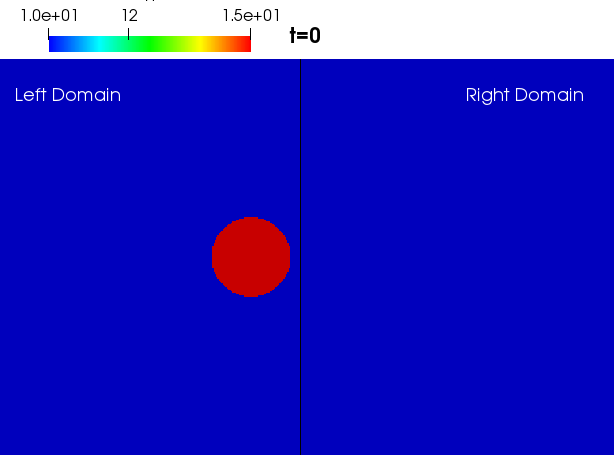
\includegraphics[scale=0.22]{./Resources/Images/unidirectional0_g_0.png}
%\caption{sadf}
%\end{figure}
\end{textblock*}

\begin{figure}[htp]
\centering
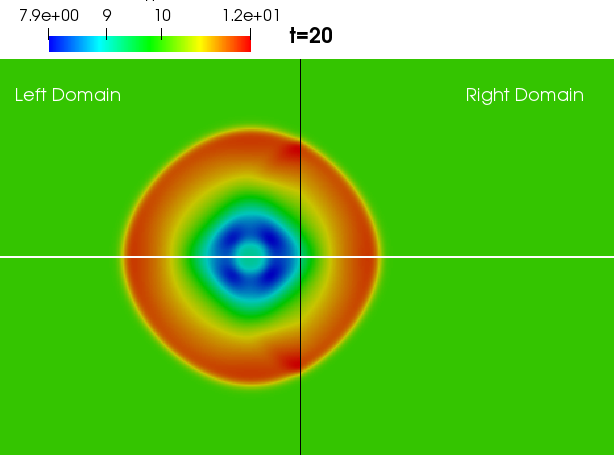
\includegraphics[width=.25\textwidth]{./Resources/Images/unidirectional20_g_0.png}\hfill
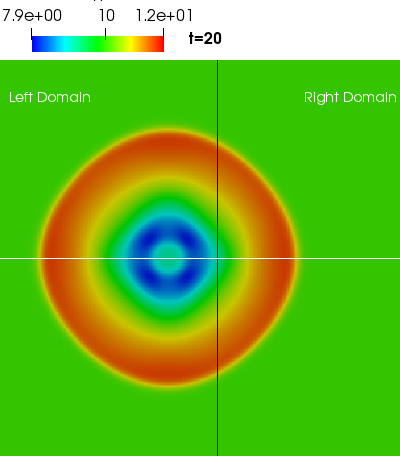
\includegraphics[width=.25\textwidth]{./Resources/Images/unidirectional20_g_bueno.png}\hfill
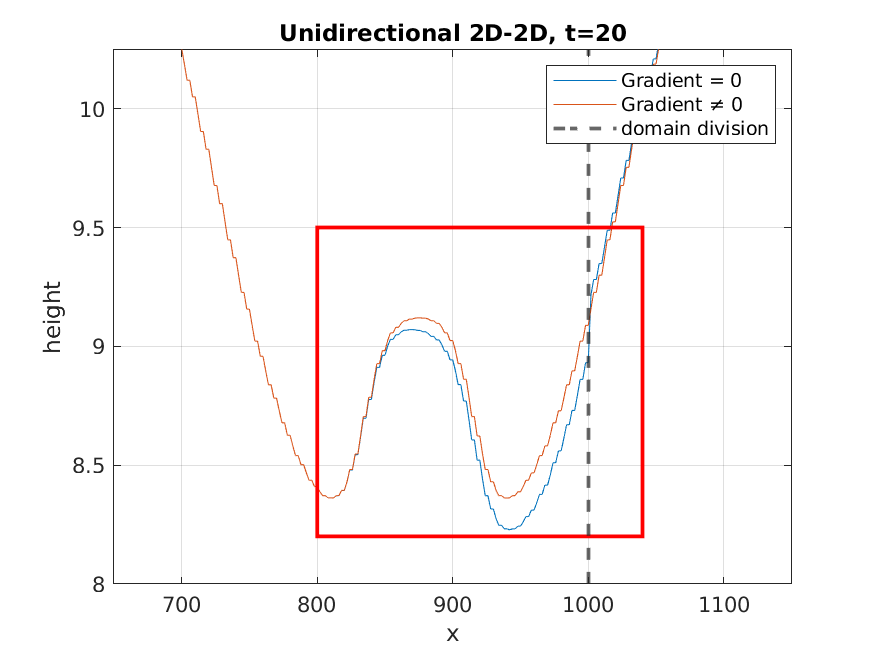
\includegraphics[width=.4\textwidth]{./Resources/Images/unidirectional_graph.png}

\caption{Top right: $h(t=0)$. Left: $h(t=20), \nabla_\eta=0$. Middle: $h(t=20),\nabla_\eta \neq0$. Right: graphed values at the middle of the domain}
\end{figure}

\end{frame}


%%%%%%%%%%%%%%%%%%
%%%%%%%%%%%%%%%%%%
\begin{frame}
\shiftedframetitle{Current Status}
\vspace{-0.5cm}
{\large \hspace{3mm} $2D$ SWE - $2D$ SWE Bidirectional}\\
Case: Radial dam break, no bathymetry
\begin{textblock*}{1cm}(17cm,1pt) % {block width} (coords)
%\begin{figure}
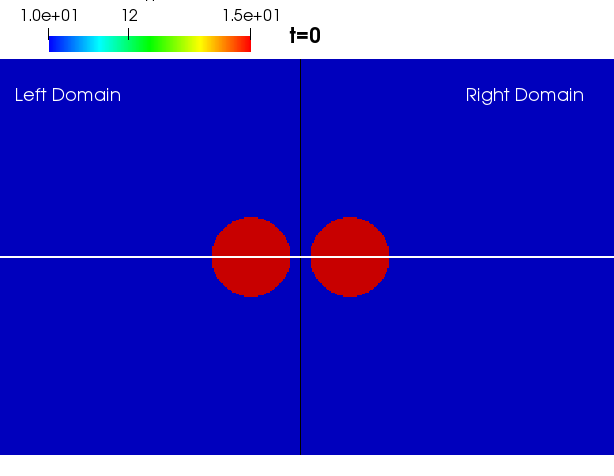
\includegraphics[scale=0.22]{./Resources/Images/bidirectional0_g_0.png}
%\caption{sadf}
%\end{figure}
\end{textblock*}

\begin{figure}[htp]
\centering
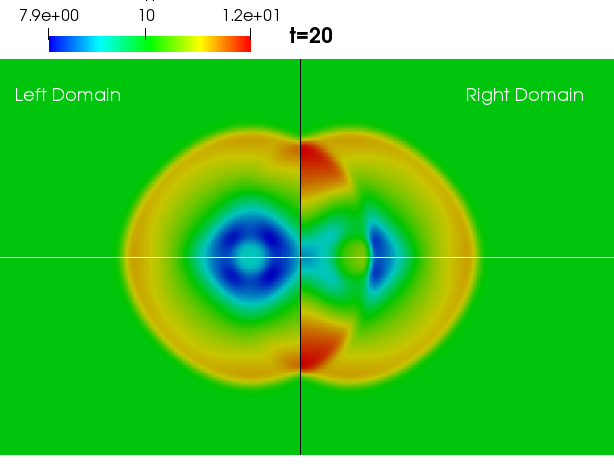
\includegraphics[width=.25\textwidth]{./Resources/Images/bidirectional20_g_0.png}\hfill
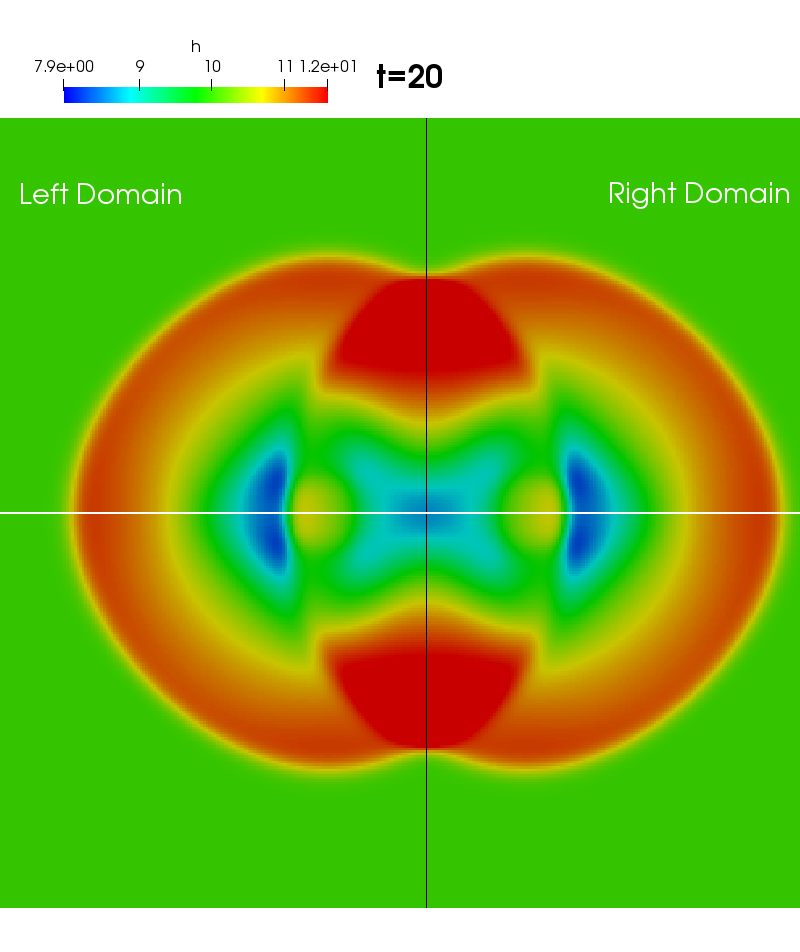
\includegraphics[width=.25\textwidth]{./Resources/Images/bidirectional20_g_bueno.png}\hfill
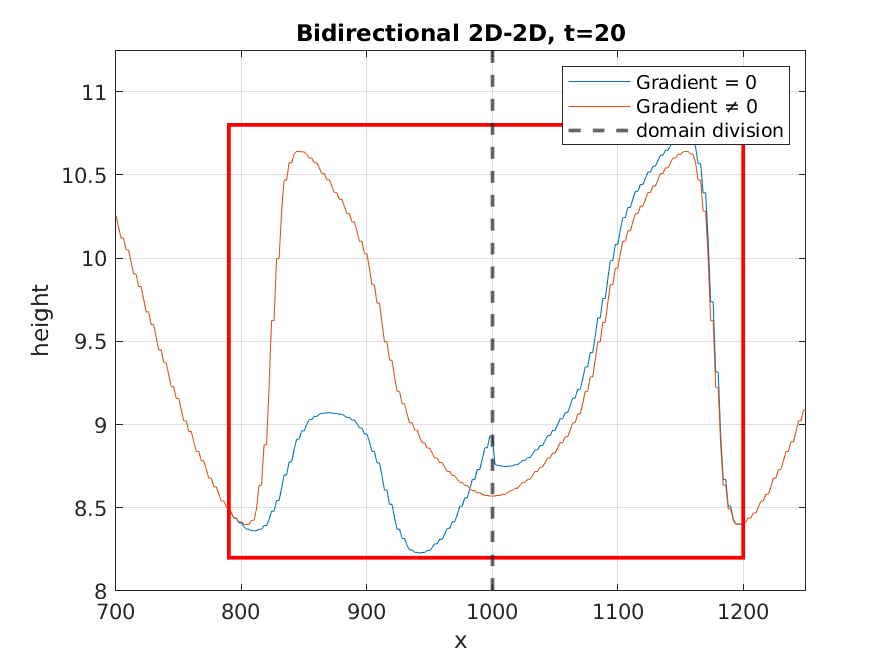
\includegraphics[width=.4\textwidth]{./Resources/Images/bidirectional_graph.png}
\caption{Top right: $h(t=0)$. Left: $h(t=20),\nabla_\eta=0$. Middle: $h(t=20)$,$\nabla_\eta \neq0$. Right: graphed values at the middle of the domain}
\end{figure}

\end{frame}

%%%%%%%%%%%%%%%%%%
%%%%%%%%%%%%%%%%%%
%\begin{frame}
%\shiftedframetitle{Current Status}
%\vspace{-0.5cm}
%{\large \hspace{3mm} 2D SWE - 2D SWE Bidirectional}\\
%Case: Radial Dam Break, Bathymetry = 0, Top: gradient $\neq 0$. Bottom: gradient $=0$
%\begin{multicols}{2}
%
%\begin{figure}
%\includegraphics[scale=0.15]{./Resources/Images/bidirectional0.png}%
%\end{figure}
%
%\begin{figure}
%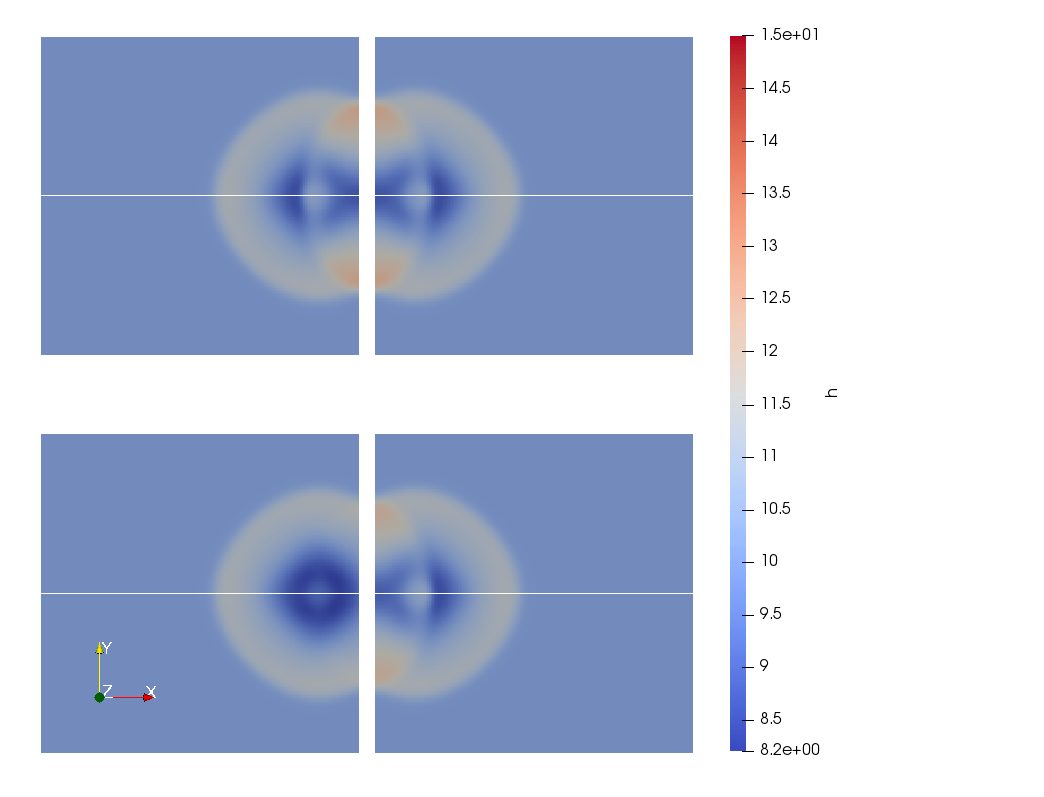
\includegraphics[scale=0.15]{./Resources/Images/bidirectional.png}%
%\end{figure}
%
%\vfill\columnbreak
%
%\begin{figure}
%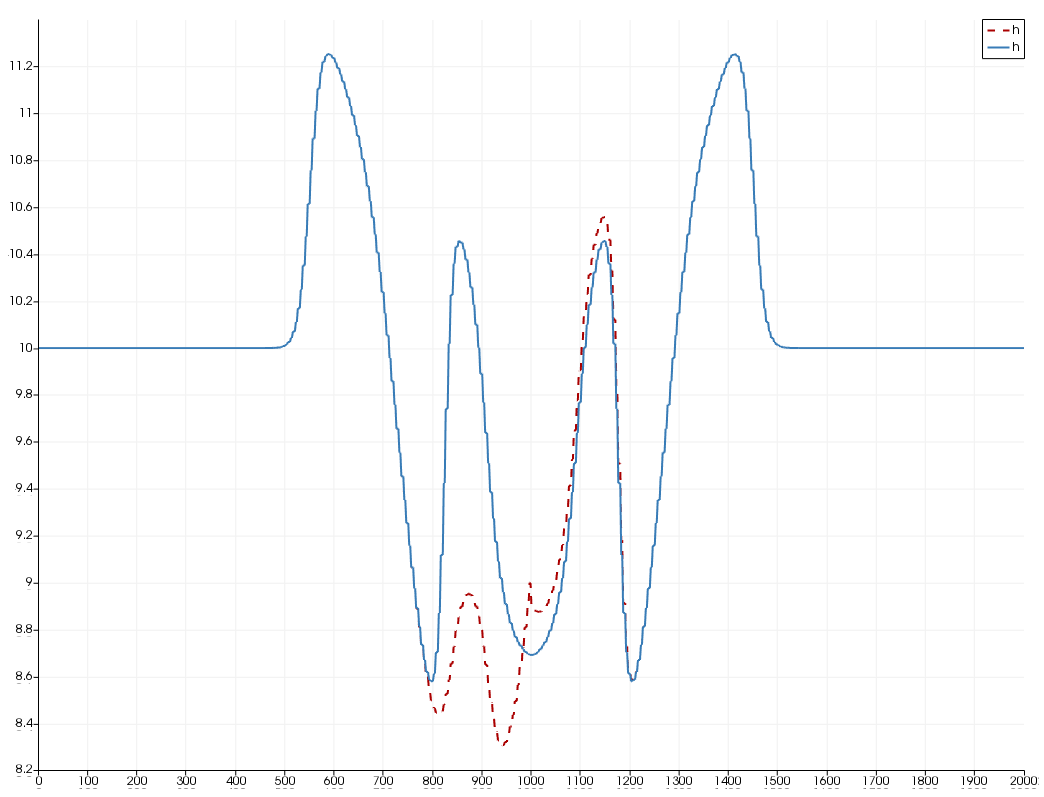
\includegraphics[scale=0.32]{./Resources/Images/bidirectional_lines.png}%
%\end{figure}
%\end{multicols}
%
%\end{frame}



%%%%%%%%%%%%%%%%%%
%%%%%%%%%%%%%%%%%%
\begin{frame}
\shiftedframetitle{TO-DOs}

\begin{figure}
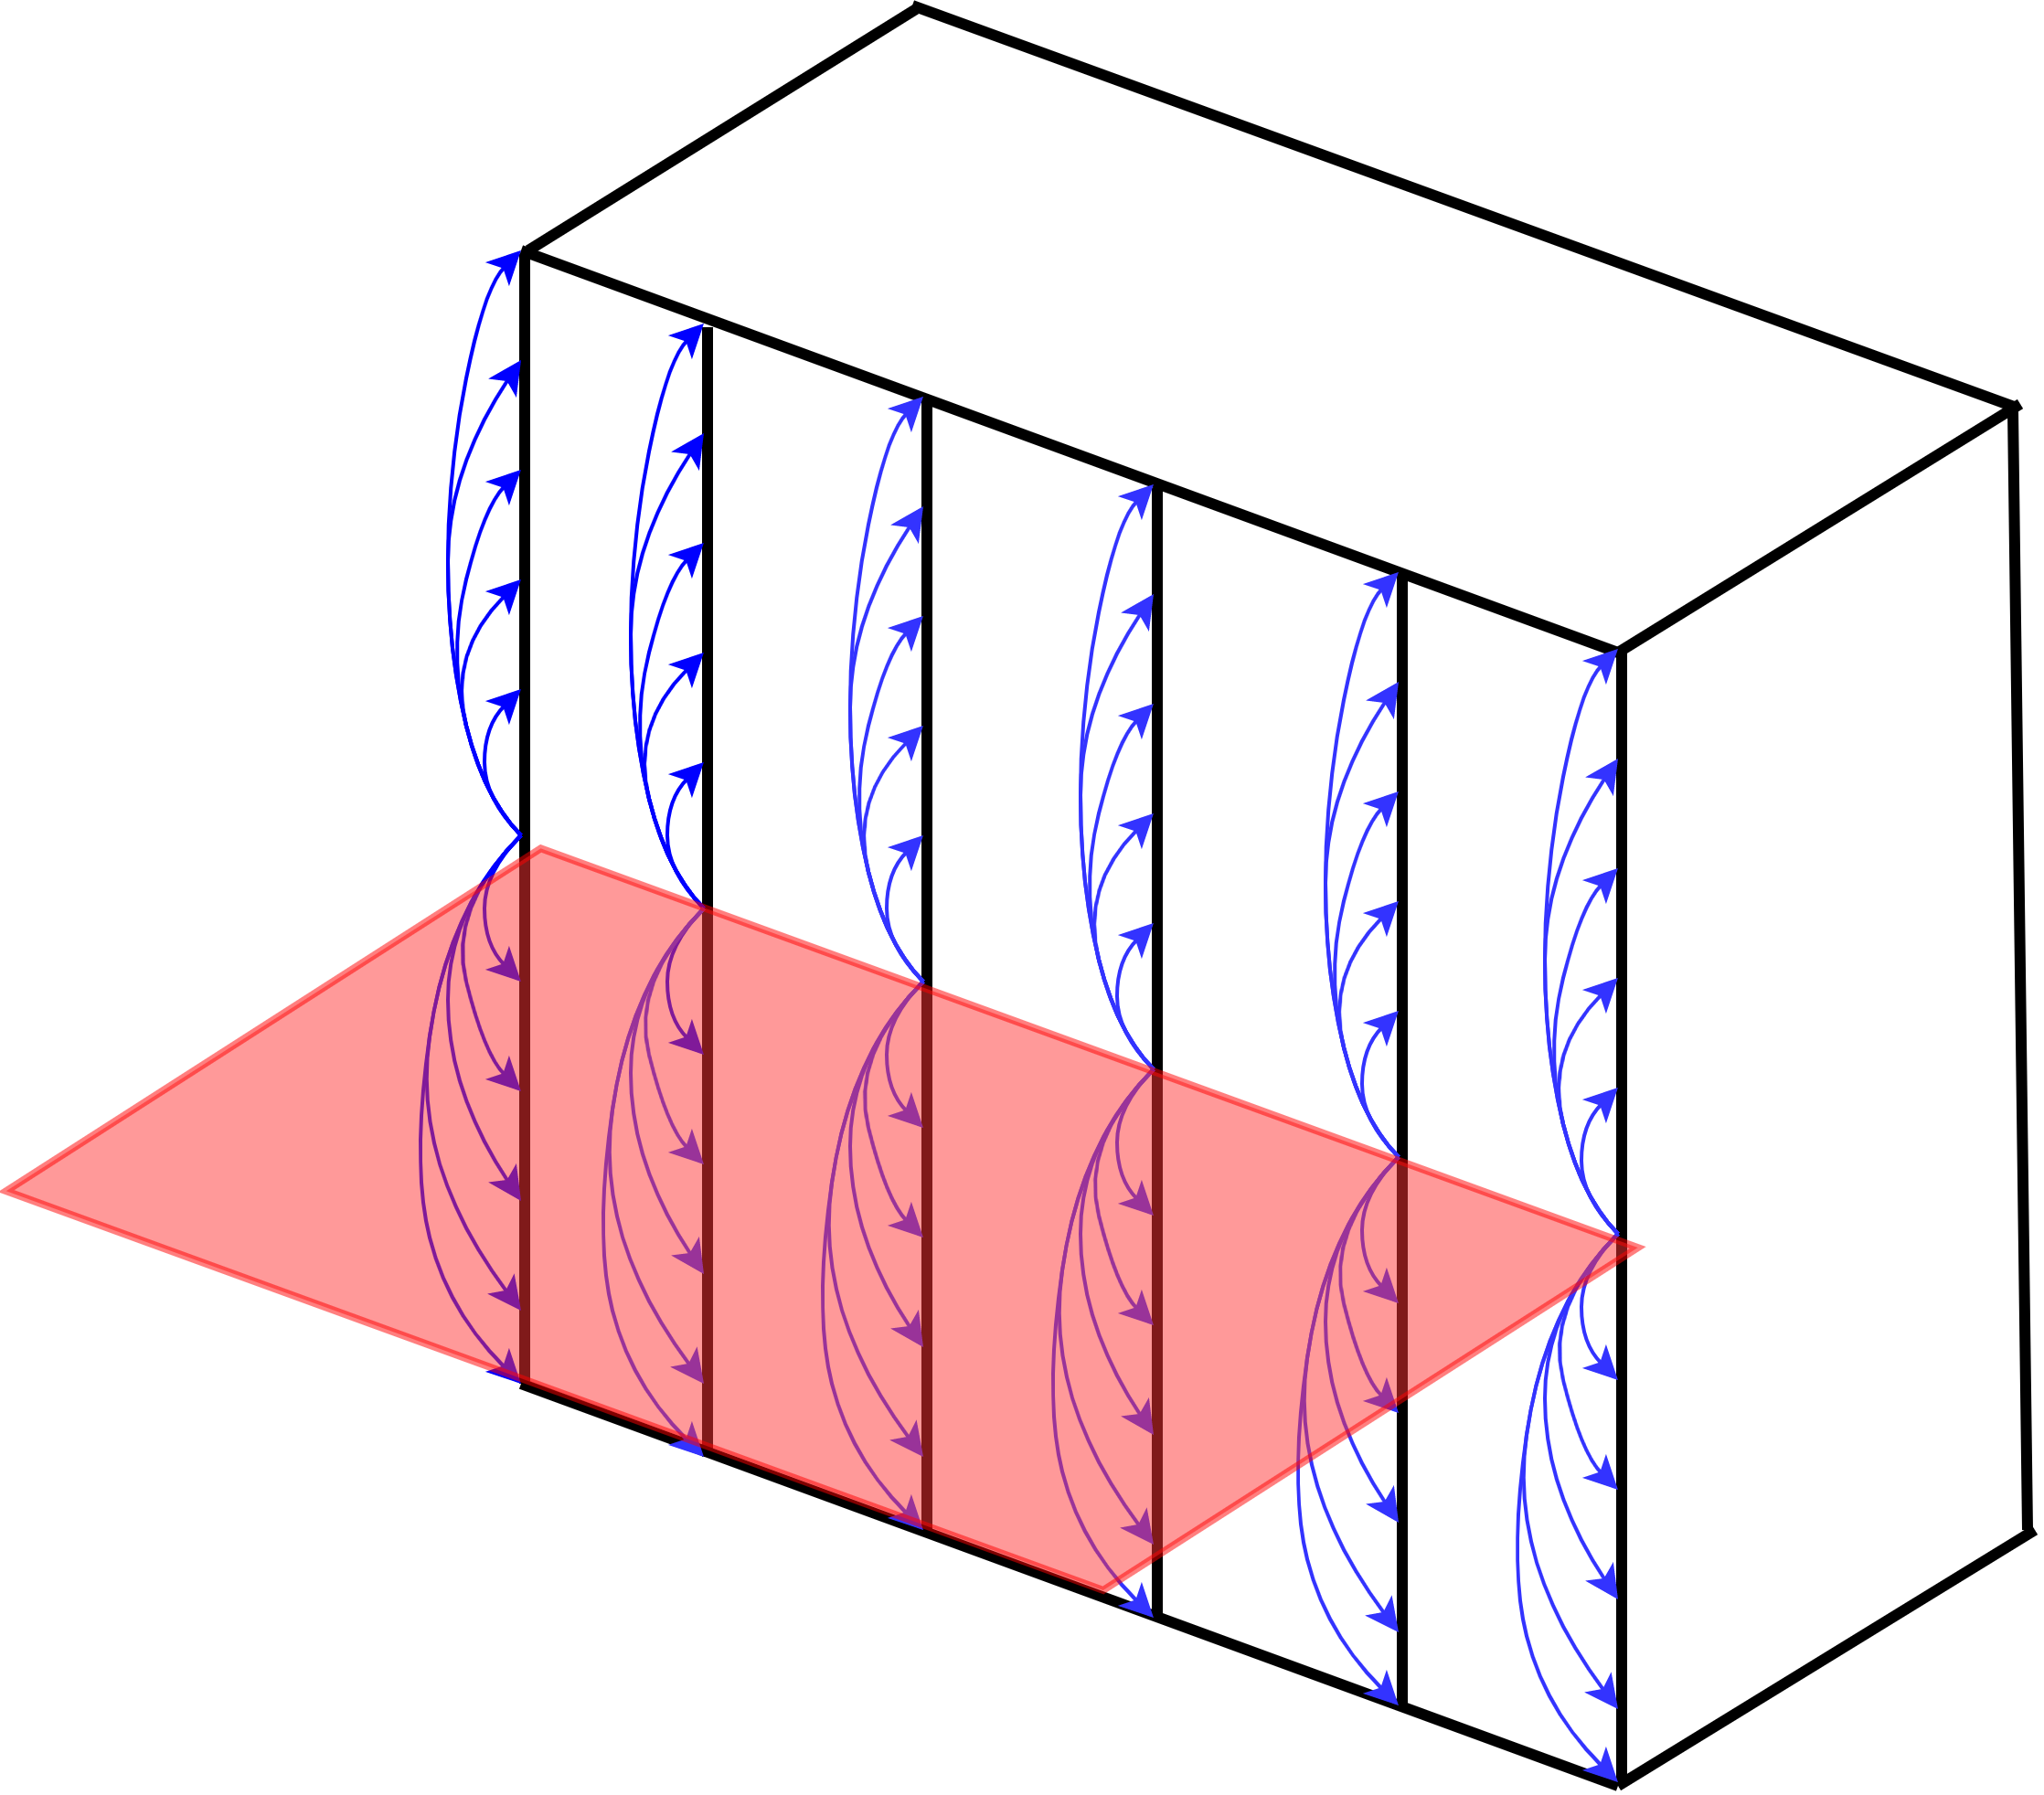
\includegraphics[scale=0.5]{./Resources/Images/mapping23.png}%
\end{figure}

\end{frame}


%%%%%%%%%%%%%%%%%%
%%%%%%%%%%%%%%%%%%
\begin{frame}
\shiftedframetitle{TO-DOs}

\begin{figure}
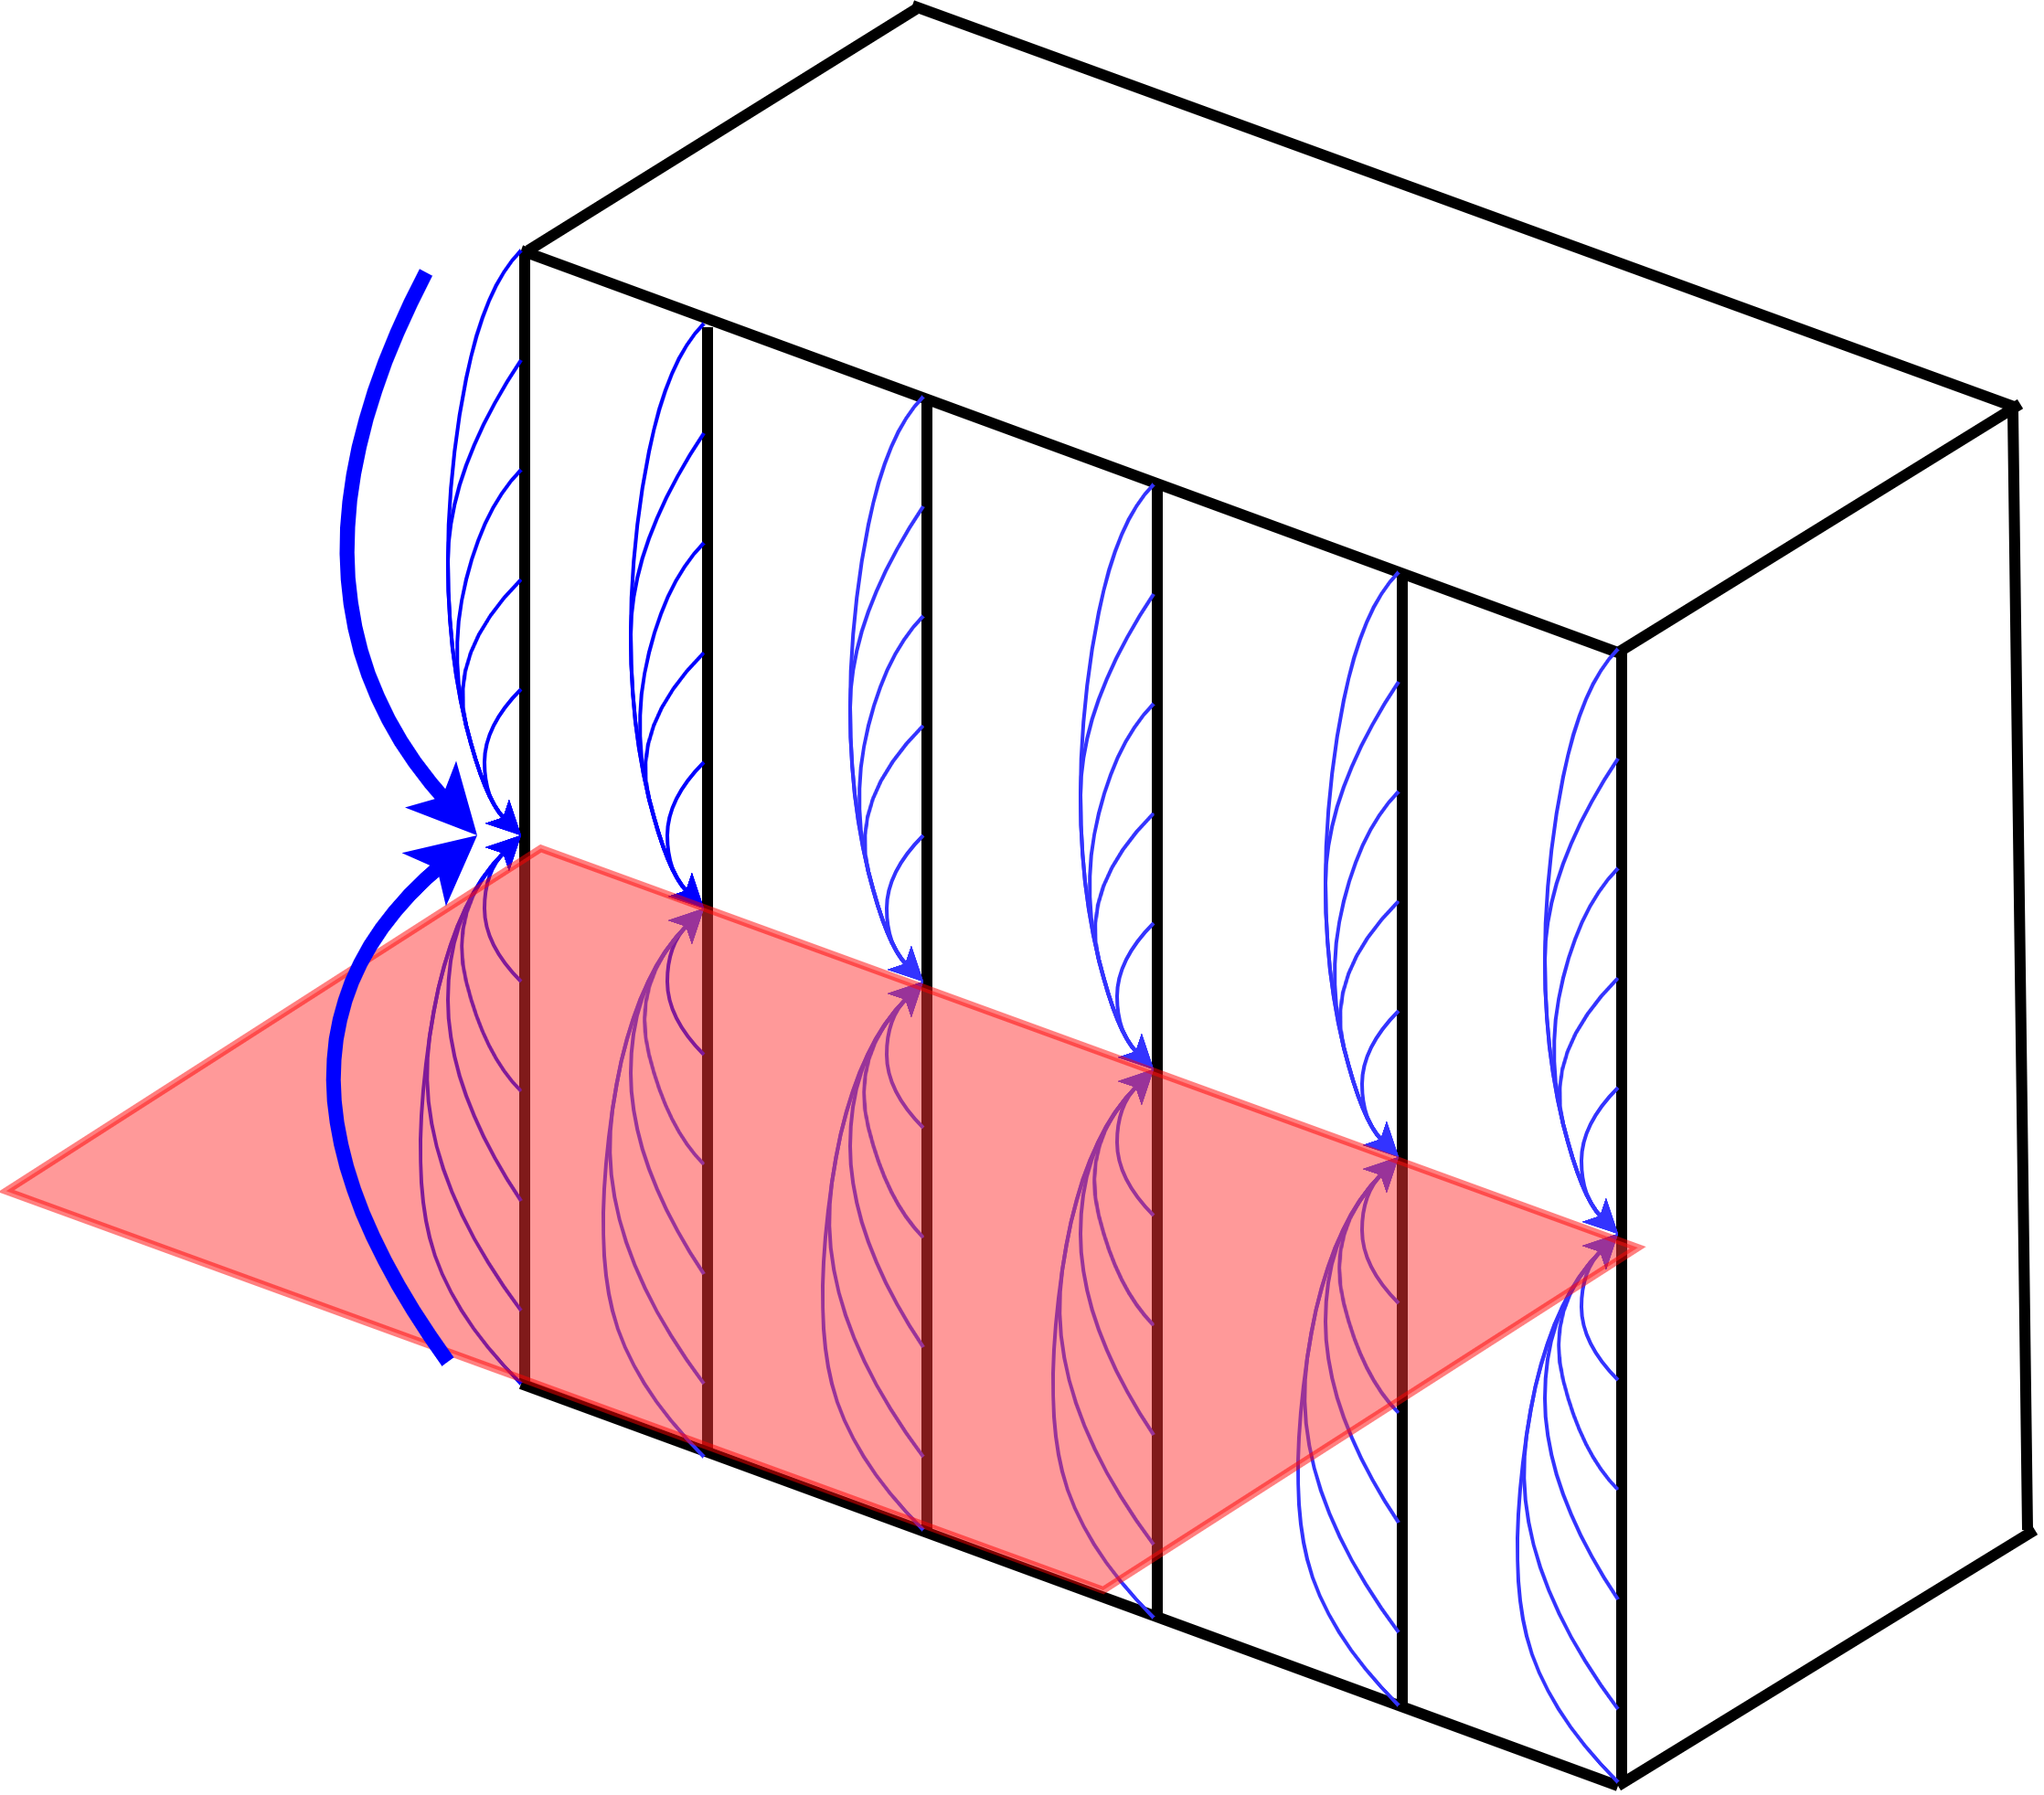
\includegraphics[scale=0.5]{./Resources/Images/mapping32.png}%
\caption{mapping $3D$ to $2D$}
\end{figure}

\end{frame}


%%%%%%%%%%%%%%%%%%%%
%%% Folie: Farben %%
%%%%%%%%%%%%%%%%%%%%
%\begin{frame}
%    \shiftedframetitle{Farben}
%    
%Als erstes soll mit schwarz und weiß gearbeitet werden.\newline
%Für Aufwändigere Darstellungen sind Farben mit Bedacht und in möglichst
%geringem Umfang einzusetzen.
%
%In diesem Folienmaster ist die Farbpalette festgelegt.
%
%{
%    \renewcommand{\arraystretch}{1.2} % skaliert die Tabellen mit Farbfeldern
%
%    Zuerst mit den Primärfarben arbeiten.
%
%    \setlength{\fboxsep}{-1pt} \setlength{\fboxrule}{1pt} % fbox/framebox konfigurieren
%
%    \vspace*{-5mm}
%    \begin{tabularx}{\textwidth}{@{} l @{\hspace{4mm}} l @{\hspace{4mm}} l}
%        \crule[TUMBlau]{24mm}{6mm}
%        & \crule[black]{24mm}{6mm}
%        & \fbox{\crule[white]{24mm}{6mm}}
%    \end{tabularx}
%
%    \vspace*{-5mm}
%    Für z.B. komplexe Diagramme stehen noch Sekundärfarben zur Verfügung.
%
%    \vspace*{-5mm}
%    \begin{tabularx}{\textwidth}{@{} l @{\hspace{4mm}} l @{\hspace{4mm}} l @{\hspace{4mm}} l}
%        \crule[TUMBlauDunkel]{24mm}{6mm}
%        & \crule[TUMBlauMittel]{24mm}{6mm}
%        & \crule[TUMBlauHell]{24mm}{6mm}
%        & \crule[TUMGrau]{24mm}{6mm}
%    \end{tabularx}
%
%    \vspace*{-5mm}
%    Bei weiterer Komplexität oder zusätzlichen Markierungen:
%
%    \vspace*{-5mm}
%    \begin{tabularx}{\textwidth}{@{} l @{\hspace{4mm}} l @{\hspace{4mm}} l }
%        \crule[TUMOrange]{24mm}{6mm}
%        & \crule[TUMGruen]{24mm}{6mm}
%        & \crule[TUMElfenbein]{24mm}{6mm}
%    \end{tabularx}
%}
%
%\end{frame}
%\clearpage
%
%
%%%%%%%%%%%%%%%%%%%
%%% Folie: Texte %%
%%%%%%%%%%%%%%%%%%%
%\begin{frame}
%    \shiftedframetitle{Texte}
% 
%Kurze und knappe Texte, Fließtexte linksbündig, kein Blocksatz \\[\baselineskip]
%
%Beispiel:\newline
%Tem soluptam, nisi as verum ereprehendam at acculpa quidisq uissit volupta
%tusdant utem as etur, odi odis es doluptiae dem nimaion con nossinctenis pora
%quam voloria consenimus blabore everfer epeliquo maio etur.
%
%\end{frame}
%\clearpage
%
%
%
%
%%%%%%%%%%%%%%%%%%%%%%%%%%%%%%%
%% Folie: Bilder - Allgemein %%
%%%%%%%%%%%%%%%%%%%%%%%%%%%%%%%
%\begin{frame}
%    \shiftedframetitle{Bilder -- Allgemein}
%    
%schlichte Darstellung von Informationen \\[\baselineskip]
%
%reduzierte Farben \\[\baselineskip]
%
%Rahmen und Überlagerungen nach Möglichkeit vermeiden \\[\baselineskip]
%
%    
%\end{frame}
%\clearpage
%
%
%%%%%%%%%%%%%%%%%%%%%%%%%%
%% Folie: Bilder - Zwei %%
%%%%%%%%%%%%%%%%%%%%%%%%%%
%\begin{frame}
%    \shiftedframetitle{Bilder}
%    
%Bildbeschreibung\newline
%oberer Bildrand: Begrenzung durch Text\\[\baselineskip]
%
%\mbox{
\includegraphics[height=.5\paperheight, trim=0cm 14cm 0cm 0cm, clip=true]{./Resources/Images/SternenhimmelHochkant.jpg}}%
%\hspace{6.5mm}%
%\mbox{
\includegraphics[height=.5\paperheight, trim=0cm 14cm 0cm 0cm, clip=true]{./Resources/Images/SternenhimmelHochkant.jpg}}
%
%\end{frame}
%\clearpage
%
%
%%%%%%%%%%%%%%%%%%%%%%%%%%%%%%%%%%%%%%%%
%% Folie: Bilder - Zweispaltige Seite %%
%%%%%%%%%%%%%%%%%%%%%%%%%%%%%%%%%%%%%%%%
%\begin{frame}
%    \shiftedframetitle{Bilder}
%
%\begin{multicols}{2}
%    \textbf{Überschrift 2}\newline
%    Hier steht ein einleitender oder beschreibender Fließtext und nach Wunsch
%    eine Aufzählung.
%
%    Punkt 1
%
%    Punkt 2
%
%    Punkt 3
%
%    Punkt 4
%    \vfill\columnbreak
%    
\includegraphics[width=\columnwidth, height=.7\textheight]{./Resources/Images/SternenhimmelHochkant.jpg}%
%\end{multicols}
%    
%\end{frame}
%\clearpage
%
%
%%%%%%%%%%%%%%%%%%%%%%%%%%%%%%%
%% Folie: Bilder - Textbreit %%
%%%%%%%%%%%%%%%%%%%%%%%%%%%%%%%
%\begin{frame}
%    \shiftedframetitle{Bilder}
%
%Bildbeschreibung\newline
%oberer Bildrand: Begrenzung durch Text\\[\baselineskip]
%
%
\includegraphics[width=\textwidth, height=.55\textheight]{./Resources/Images/SternenhimmelQuer.jpg}%
%
%\end{frame}
%\clearpage
%
%%%%%%%%%%%%%%%%%%%%%%%%%%%%%%%%%%%%%%%%%%%%%%%%%%
%% Folie: Bilder - seitenbreit mit Beschreibung %%
%%%%%%%%%%%%%%%%%%%%%%%%%%%%%%%%%%%%%%%%%%%%%%%%%%
%\begin{frame}
%    \shiftedframetitle{Bilder}
%
%    Bildbeschreibung\newline
%    oberer Bildrand: Begrenzung durch Text
%
%\vspace*{-3mm}
%\begin{minipage}[t][0cm]{\paperwidth}%
%\hspace*{-\PraesentationSeitenrand}%
%
\includegraphics[width=\paperwidth]{./Resources/Images/SternenhimmelQuer.jpg}
%\end{minipage}
%    
%\end{frame}
%\clearpage
%
%%%%%%%%%%%%%%%%%%%%%%%%%%%%%%%%%%%%%%%%%%%%%%%%%%%%%
%% Folie: Nicht Format füllende Bilder %%
%%%%%%%%%%%%%%%%%%%%%%%%%%%%%%%%%%%%%%%%%%%%%%%%%%%%%
%\begin{frame}
%    \shiftedframetitle{Nicht Format füllende Bilder}
%    
%    Weißer bzw. transparenter Hintergrund\newline
%    mit genug Freiraum anordnen
%
%
%\begin{textblock*}{0.4\paperwidth}[0,1](0cm, \textheight - \PraesentationSeitenrand)%
%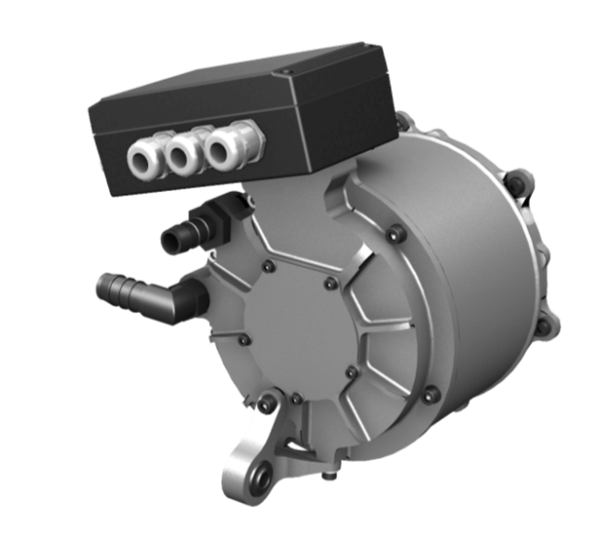
\includegraphics[width=0.4\paperwidth]{./Resources/Presentation/Images/Motor.png}
%\end{textblock*}
%
%\begin{textblock*}{0.6\paperwidth}[1,1](\textwidth + \PraesentationSeitenrand, \textheight - \PraesentationSeitenrand)%
%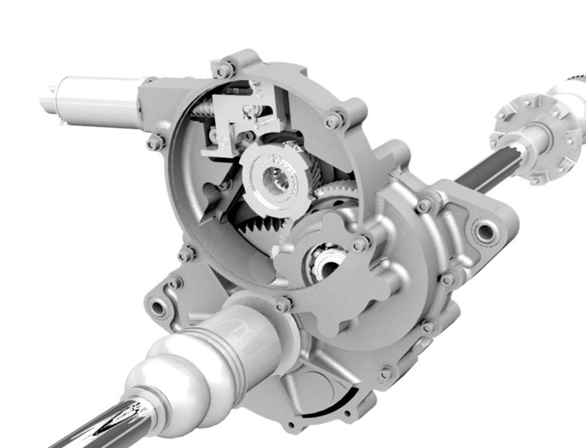
\includegraphics[width=0.6\paperwidth]{./Resources/Presentation/Images/Getriebe.png}
%\end{textblock*}
%
%\end{frame}
%\clearpage
%
%
%%%%%%%%%%%%%%%%%%%%%%%%%%%%%%%%%%%
%% Folie: Bilder - formatfüllend %%
%%%%%%%%%%%%%%%%%%%%%%%%%%%%%%%%%%%
%\begin{frame}
%    \shiftedframetitle{Bilder Format füllend -- maximale Bildgröße}
%
%\begin{minipage}[t][0cm]{\paperwidth}%
%\hspace*{-\PraesentationSeitenrand}%
%
\includegraphics[width=\textwidth]{./Resources/Images/SternenhimmelQuer.jpg}
%\end{minipage}
%    
%\end{frame}
%\clearpage
%
%%%%%%%%%%%%%%%%%%%%%%%%%%%%%%%%%%%%%%%%%%%%%%%%%%%%%%
%%% Folie: Nicht Format füllende Bilder %%
%%%%%%%%%%%%%%%%%%%%%%%%%%%%%%%%%%%%%%%%%%%%%%%%%%%%%%
%\begin{frame}
%    \shiftedframetitle{Nicht Format füllende Bilder}
%    
%Alternativ mit formatfüllendem Hintergrund: Weiß 5\% dunkler\newline
%Beschriftungen können zusätzlich neben den Bildern angebracht werden
%
%\begin{textblock*}{\paperwidth}[0,0](0cm, .4\textheight)%
%Bilderklärung
%\end{textblock*}
%
%\begin{textblock*}{\paperwidth}[1,0](\textwidth, .4\textheight)%
%\raggedleft%
%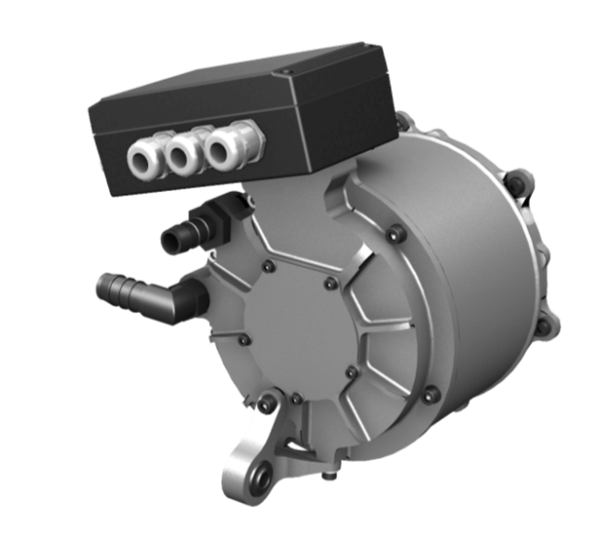
\includegraphics[height=0.5\textheight]{./Resources/Presentation/Images/Motor.png}
%\end{textblock*}
%
%\end{frame}
%\clearpage
%
%
%%%%%%%%%%%%%%%%%%%%%%%%%%%%%%%%%%%%%%%%%%%%%%%%%%%%%
%% Folie: Tabelle - Ohne Rand 					   %%
%%%%%%%%%%%%%%%%%%%%%%%%%%%%%%%%%%%%%%%%%%%%%%%%%%%%%
%\begin{frame}
%    \shiftedframetitle{Tabelle -- Beispiel 1}
%    
%Tabelle ohne Farbe und kein Rand \\
%innerer Seitenrand links 0 cm, um Faktor 1,75 skalierte Tabelle (für genug Zeilenabstand)
%
%\raggedright
%{
%    \vspace*{0.3pt}
%    \renewcommand{\arraystretch}{1.75} % skaliert die Tabelle auf die gewünschte Größe
%    \begin{tabularx}{\textwidth}{@{} l @{\hspace{38.7mm}} l}
%        Ø - Strecke & 39 km/Tag (14.360 km/Jahr) \\
%        Ø - Geschwindigkeit & 25 km/h \\
%        Ø - Verfügbare Ladezeit & 22 h/Tag \\
%        Kosten   & Kleinwagen mit Verbrennungsmotor \\
%        Einsatzgebiet   &  Stadt und Umland
%    \end{tabularx}
%}
%\end{frame}
%
%
%%%%%%%%%%%%%%%%%%%%%%%%%%%%%%%%%%%%%%%%%%%%%%%%%%%%%%
%%% Folie: Tabelle - Mit Rand                       %%
%%%%%%%%%%%%%%%%%%%%%%%%%%%%%%%%%%%%%%%%%%%%%%%%%%%%%%
%\begin{frame}
%    \shiftedframetitle{Tabelle -- Beispiel 2}
%    
%Tabelle ohne Farbe und mit Rand\\
%automatische Zelleninnenabstände, um Faktor 1,75 skalierte Tabelle (für genug Zeilenabstand)
%
%\raggedright
%{
%    \vspace*{0.3pt}
%    \renewcommand{\arraystretch}{1.75} % skaliert die Tabelle auf die gewünschte Größe
%    \begin{tabularx}{\textwidth}{| l @{\hspace{38.7mm}} | X |}
%        \hline
%        Ø - Strecke & 39 km/Tag (14.360 km/Jahr) \\ \hline
%        Ø - Geschwindigkeit & 25 km/h \\ \hline
%        Ø - Verfügbare Ladezeit & 22 h/Tag \\ \hline
%        Kosten   & Kleinwagen mit Verbrennungsmotor \\ \hline
%        Einsatzgebiet   &  Stadt und Umland \\ \hline
%    \end{tabularx}
%}
%\end{frame}
%
%\clearpage
%
%
%%%%%%%%%%%%%%%%%%%%%%%%%%%%%%%%%%%%%%%%%%%%%%%%%%%%%%
%%% Folie: Diagramme - Beispiel 1                   %%
%%%%%%%%%%%%%%%%%%%%%%%%%%%%%%%%%%%%%%%%%%%%%%%%%%%%%%
%\begin{frame}
%    \shiftedframetitle{Diagramme -- Beispiel 1}
%
%%Nach Möglichkeit linksbündig bleiben \\
%%Unnötige Striche und Balken vermeiden
%
%\begin{center}%
%    \vspace*{-1cm}
%   \begin{tikzpicture}
%        \begin{axis}[
%                % kein Abstand zwischen Balken:
%                xbar=0,
%                draw opacity=0,
%                bar width=14,
%                axis x line=none,
%                axis line style={transparent},
%                every tick/.style={transparent},
%                xmin=0,
%                width=\textwidth,
%                height=.6\textheight,
%                enlarge y limits=0.15,
%                symbolic y coords={Kategorie 4,Kategorie 3,Kategorie 2,Kategorie 1},
%                ytick=data,
%                legend image code/.code={\draw[draw=none] (0cm,-0.12cm) rectangle (0.29cm,0.17cm);}, % Legenden-Symbol  
%                legend columns=3,
%                reverse legend,
%                legend style={
%                    fill=none,
%                    draw=none,
%                    /tikz/every odd column/.append style={column sep=0.07cm}, % Abstand zwischen Legenden-Symbol und Text
%                    /tikz/every even column/.append style={column sep=0.8cm} % Abstand zwischen den Legendeneinträgen
%                 },
%                 legend to name=PraesentationDiagrammHorizontalLegende
%            ]
%            
%            \addlegendentry{Datenreihe 3}
%            \addlegendentry{Datenreihe 2}
%            \addlegendentry{Datenreihe 1}
%            
%            \addplot[color=TUMBlauMittel, fill=TUMBlauMittel] coordinates {
%                (1.2,Kategorie 1)
%                (1.6,Kategorie 2)
%                (2.2,Kategorie 3)
%                (3.4,Kategorie 4)
%            };
%            
%            \addplot[color=TUMBlauHell, fill=TUMBlauHell] coordinates {
%                (1.5,Kategorie 1)
%                (3.0,Kategorie 2)
%                (1.0,Kategorie 3)
%                (2.0,Kategorie 4)
%            };
%                
%            \addplot[color=TUMBlauDunkel, fill=TUMBlauDunkel] coordinates {
%                (3.0,Kategorie 1)
%                (2.0,Kategorie 2)
%                (2.5,Kategorie 3)
%                (3.0,Kategorie 4)
%            };
%        \end{axis}
%    \end{tikzpicture}
%
%    \vspace*{-5mm}
%    \ref*{PraesentationDiagrammHorizontalLegende}%
%\end{center}
%\end{frame}
%\clearpage
%
%
%%%%%%%%%%%%%%%%%%%%%%%%%%%%%%%%%%%%%%%%%%%%%%%%%%%%%%
%%% Folie: Diagramme                                %%
%%%%%%%%%%%%%%%%%%%%%%%%%%%%%%%%%%%%%%%%%%%%%%%%%%%%%%
%\begin{frame}
%    \shiftedframetitle{Diagramme}
%
%\begin{center}
%    \begin{tikzpicture}
%        \begin{axis}[
%                ybar=9.5,
%                bar width=27.1,
%                axis line style={transparent},
%                every tick/.style={transparent},
%                enlarge x limits=0.145, % X-Achse skalieren
%                clip limits=true,
%                ymin=0,
%                ymax=6,
%                width=\textwidth,
%                height=.65\textheight,
%                symbolic x coords={Kategorie 1,Kategorie 2,Kategorie 3,Kategorie 4},
%                xticklabels={Kategorie 1,Kategorie 2,Kategorie 3,Kategorie 4},
%                xtick=data,
%                ytick={0,1,2,3,4,5,6},
%                every tick label/.append style={font=\fontsize{13}{14}\selectfont},
%                ymajorgrids,
%                legend image code/.code={\draw[draw=none] (0cm,-0.12cm) rectangle (0.29cm,0.17cm);}, % Legenden-Symbol  
%                legend columns=3,
%                reverse legend,
%                legend style={
%                    font={\usebeamerfont{footnote}},
%                    fill=none,
%                    draw=none,
%                    /tikz/every odd column/.append style={column sep=0.07cm}, % Abstand zwischen Legenden-Symbol
%                    /tikz/every even column/.append style={column sep=0.8cm} % Abstand zwischen den Legendeneinträgen
%                 },
%                legend to name=PraesentationDiagrammVertikalLegende
%            ]
%            
%            \addlegendentry{Datenreihe 3}        
%            \addlegendentry{Datenreihe 2}    
%            \addlegendentry{Datenreihe 1}    
%            
%            \addplot[color=TUMBlauDunkel, fill=TUMBlauDunkel] coordinates {
%                (Kategorie 1,4.2)
%                (Kategorie 2,2.5)
%                (Kategorie 3,3.5)
%                (Kategorie 4,4.5)
%            };
%            
%            \addplot[color=TUMBlauHell, fill=TUMBlauHell] coordinates {
%                (Kategorie 1,2.3)
%                (Kategorie 2,4.5)
%                (Kategorie 3,1.8)
%                (Kategorie 4,2.8)
%            };
%            
%            \addplot[color=TUMBlauMittel, fill=TUMBlauMittel] coordinates {
%                (Kategorie 1,2.0)
%                (Kategorie 2,2.0)
%                (Kategorie 3,3.0)
%                (Kategorie 4,5.0)
%            };        
%        \end{axis}
%    \end{tikzpicture}
%
%    \vspace*{-5mm}
%    \ref*{PraesentationDiagrammVertikalLegende}%
%\end{center}
%\end{frame}
%\clearpage
%
